\documentclass[12pt,a4paper]{article}
\usepackage{geometry}
\geometry{left=2.5cm,right=2.5cm,top=2.0cm,bottom=2.5cm}
\usepackage[english]{babel}
\usepackage{amsmath,amsthm,mathtools}
\usepackage{amsfonts}
\usepackage[longend,ruled,linesnumbered]{algorithm2e}
\usepackage{fancyhdr}
\usepackage{ctex}
\usepackage{array}
\usepackage{listings}
\usepackage{color}
\usepackage{graphicx}
\usepackage{amssymb}
\newtheorem{theorem}{定理}
\newtheorem{lemma}[theorem]{引理}
\newtheorem{corollary}[theorem]{推论}
\usepackage{listings}
\usepackage{xcolor}

\definecolor{codegreen}{rgb}{0,0.6,0}
\definecolor{codegray}{rgb}{0.5,0.5,0.5}
\definecolor{codepurple}{rgb}{0.58,0,0.82}
\definecolor{backcolour}{rgb}{0.95,0.95,0.92}

\lstdefinestyle{mystyle}{
	backgroundcolor=\color{backcolour},
	commentstyle=\color{codegreen},
	keywordstyle=\color{magenta},
	numberstyle=\tiny\color{codegray},
	stringstyle=\color{codepurple},
	basicstyle=\ttfamily\footnotesize,
	breakatwhitespace=false,
	breaklines=true,
	captionpos=b,
	keepspaces=true,
	numbers=left,
	numbersep=5pt,
	showspaces=false,
	showstringspaces=false,
	showtabs=false,
	tabsize=2
}

\lstset{style=mystyle}

\begin{document}
	
	\section*{大作业报告}
	
	在方形区域$\Omega=[0,1]^2$和L型区域$\Omega=[-1,1]^2 \textbackslash [0,1]^2 $上,使用Lagrange二次元求解问题
	$$\begin{cases}-\Delta u+2u=f\triangleq(2+2\pi^2)\sin(\pi x_1)\sin(\pi x_2)\\u|_{\partial\Omega}=0\end{cases}$$
	该问题真解为$u(x_1,x_2)=\sin(\pi x_1)\sin(\pi x_2)$.
	
	变分形式:
	
	找$u \in H_0^1(\Omega)$,使得对于$\forall v \in H_0^1(\Omega)$,有
	
	$$
	\int_\Omega \nabla u \nabla v + 2uv dx= \int_\Omega fv dx
	$$
	
	令$V_{h0}=\{v\in H_0^1(\Omega)\mid v|_K\in P_2(K),\forall K\in \Gamma_h\}$
	
	有限元离散:
		
	找$u_h \in V_{h0}$,使得对于$\forall v_h \in V_{h0}$,有
	
	$$
	\int_\Omega \nabla u_h \nabla v_h + 2u_h v_h dx= \int_\Omega fv_h dx
	$$
	
	设$\dim V_h = M$,其基函数系为$\{\varphi_i(x)\}_{i=1}^M$,则$u_h=\sum_{i=1}^MU_i\varphi_i(x),\quad v_h=\sum_{i=1}^MV_i\varphi_i(x).$
	
	离散问题可化为有限元方程组$AU=F$,其中
	
	$$U \triangleq (U_1,U_2,\cdots,U_M)^\top$$
	$$A\triangleq\left(A_{ij}\right)_{M\times M},A_{ij}\triangleq \int_\Omega \left(\nabla \varphi_{i} \nabla \varphi_{j}+2\varphi_{i}\varphi_{j}\right)\mathrm{d}x$$
	$$F\triangleq\left(F_{1},F_{2},\cdots,F_{M}\right)^{\top},F_{i}\triangleq \int_{\Omega} f(x)\varphi_{i}(x)\mathrm{d}x$$
	
	由于解析积分通常难以计算,使用数值积分来近似积分。对于三角形单元$T$ 上的积分,可以写成:
	$$A_{ij}\approx\sum_{p=1}^{n_{quad}}w_p(\nabla\phi_i(\lambda_p)\cdot\nabla\phi_j(\lambda_p))|T|$$
	$$F_i\approx\sum_{p=1}^{n_{quad}}w_pf(\lambda_p)\phi_i(\lambda_p)|T|$$
	其中:$\lambda_p$是积分点的重心坐标,$\cdot$ $w_p$是积分点的权重,$n_{quad}$是积分点的数量,$|T|$是单元$T$的面积。
	
	MATLAB实现:
	
	\begin{lstlisting}[language=MATLAB, caption=使用有限元建立离散问题并求解的函数]
		function [u,errL2,errH1] = myfun(elem,node,pde,option)
		
		[elem2dof,edge,bdDof] = dofP2(elem);
		% important constants
		N = size(node,1);  NT = size(elem,1); NE = size(edge,1);
		Ndof = N + NE;
		
		% \nabla \lambda and |T|
		[Dlambda,area] = gradbasis(node,elem); 
		
		% generate sparse pattern
		ii = zeros(21*NT,1); 
		jj = zeros(21*NT,1); 
		index = 0;
		for i = 1:6
		for j = i:6
		ii(index+1:index+NT) = double(elem2dof(:,i)); 
		jj(index+1:index+NT) = double(elem2dof(:,j));  
		index = index + NT;
		end
		end
		
		[lambda, w] = quadpts(option.quadorder);
		nQuad = size(lambda,1);
		% compute non-zeros
		sA = zeros(21*NT,nQuad);
		for p = 1:nQuad
		% Dphi at quadrature points
		Dphip(:,:,6) = 4*(lambda(p,1)*Dlambda(:,:,2)+lambda(p,2)*Dlambda(:,:,1));
		Dphip(:,:,1) = (4*lambda(p,1)-1).*Dlambda(:,:,1);            
		Dphip(:,:,2) = (4*lambda(p,2)-1).*Dlambda(:,:,2);            
		Dphip(:,:,3) = (4*lambda(p,3)-1).*Dlambda(:,:,3);            
		Dphip(:,:,4) = 4*(lambda(p,2)*Dlambda(:,:,3)+lambda(p,3)*Dlambda(:,:,2));
		Dphip(:,:,5) = 4*(lambda(p,3)*Dlambda(:,:,1)+lambda(p,1)*Dlambda(:,:,3));
		index = 0;
		for i = 1:6
		for j = i:6
		Aij = 0;            
		Aij = Aij + w(p)*dot(Dphip(:,:,i),Dphip(:,:,j),2);
		Aij = Aij.*area;
		sA(index+1:index+NT,p) = Aij;
		index = index + NT;
		end
		end
		end
		sA = sum(sA,2);
		% assemble the matrix
		diagIdx = (ii == jj);   
		upperIdx = ~diagIdx;
		A = sparse(ii(diagIdx),jj(diagIdx),sA(diagIdx),Ndof,Ndof);
		AU = sparse(ii(upperIdx),jj(upperIdx),sA(upperIdx),Ndof,Ndof);
		A = A + AU + AU';
		
		%%%%%%%%%%%%%%%%%%%%%%%%%%%%%%%%%%%%%%%%%%%%%%%%%%%%%%%%%%%%%%%%
		% assemble the mass matrix M
		sM = zeros(21*NT, nQuad);
		for p = 1:nQuad
		phip(:,6) = 4*lambda(p,1).*lambda(p,2);
		phip(:,1) = lambda(p,1).*(2*lambda(p,1)-1);
		phip(:,2) = lambda(p,2).*(2*lambda(p,2)-1);
		phip(:,3) = lambda(p,3).*(2*lambda(p,3)-1);
		phip(:,4) = 4*lambda(p,2).*lambda(p,3);
		phip(:,5) = 4*lambda(p,3).*lambda(p,1);
		index = 0;
		for i = 1:6
		for j = i:6
		Mij = 0;
		Mij = Mij + w(p)*phip(:,i).*phip(:,j);
		Mij = Mij.*area;
		sM(index+1:index+NT,p) = Mij;
		index = index + NT;
		end
		end
		end
		sM = sum(sM,2);
		
		% assemble the mass matrix
		M = sparse(ii(diagIdx), jj(diagIdx), sM(diagIdx), Ndof, Ndof);
		MU = sparse(ii(upperIdx), jj(upperIdx), sM(upperIdx), Ndof, Ndof);
		M = M + MU + MU';
		
		% final system matrix
		A = A + 2*M;
		%%%%%%%%%%%%%%%%%%%%%%%%%%%%%%%%%%%%%%%%%%%%%%%%%%%%%%%%%%%%%%%%%%%
		
		% quadrature points in the barycentric coordinate
		[lambda,w] = quadpts(option.fquadorder);
		nQuad = size(lambda,1);
		phi(:,6) = 4*lambda(:,1).*lambda(:,2);
		phi(:,1) = lambda(:,1).*(2*lambda(:,1)-1);
		phi(:,2) = lambda(:,2).*(2*lambda(:,2)-1);
		phi(:,3) = lambda(:,3).*(2*lambda(:,3)-1);
		phi(:,4) = 4*lambda(:,2).*lambda(:,3);
		phi(:,5) = 4*lambda(:,3).*lambda(:,1);
		bt = zeros(NT,6);
		for p = 1:nQuad
		% quadrature points in the x-y coordinate
		pxy = lambda(p,1)*node(elem(:,1),:) ...
		+ lambda(p,2)*node(elem(:,2),:) ...
		+ lambda(p,3)*node(elem(:,3),:);
		
		fp = pde.f(pxy);   % function handle
		for j = 1:6
		bt(:,j) = bt(:,j) + w(p)*phi(p,j)*fp;
		end
		end
		bt = bt.*repmat(area,1,6);
		b = accumarray(elem2dof(:),bt(:),[Ndof 1]); 
		
		u = zeros(Ndof,1);
		
		% Find Dirichlet boundary dof: fixedDof
		fixedDof = []; 
		freeDof = [];
		isFixedDof = false(Ndof,1); 
		
		% isDirichlet(elem2edge(bdFlag(:)==1)) = true;
		% isFixedDof(edge(isDirichlet,:)) = true;
		% isFixedDof(N + find(isDirichlet')) = true;
		% fixedDof = find(isFixedDof);
		% freeDof = find(~isFixedDof);    
		
		fixedDof = bdDof;
		isFixedDof(fixedDof) = true;
		freeDof = find(~isFixedDof);    
		
		
		% Modify the matrix
		% Build Dirichlet boundary condition into the matrix AD by enforcing
		% |AD(fixedDof,fixedDof)=I, AD(fixedDof,freeDof)=0,
		% AD(freeDof,fixedDof)=0|.
		if ~isempty(fixedDof)
		bdidx = zeros(Ndof,1); 
		bdidx(fixedDof) = 1;
		Tbd = spdiags(bdidx,0,Ndof,Ndof);
		T = spdiags(1-bdidx,0,Ndof,Ndof);
		AD = T*A*T + Tbd;
		else
		AD = A;
		end
		
		u(freeDof) = AD(freeDof,freeDof)\b(freeDof);
		residual = norm(b - AD*u);
		
		
		
		% Dirichlet boundary conditions
		idx = (fixedDof > N);                         % index of edge nodes
		u(fixedDof(~idx)) = pde.g_D(node(fixedDof(~idx),:)); % bd value at vertex dofs
		bdEdgeIdx = fixedDof(idx) - N;
		bdEdgeMid = (node(edge(bdEdgeIdx,1),:) + node(edge(bdEdgeIdx,2),:))/2;
		u(fixedDof(idx)) = pde.g_D(bdEdgeMid);
		b = b - A*u;
		b(fixedDof) = u(fixedDof);
		
		errL2 = getL2error(node,elem,pde.exactu,u);
		errH1 = getH1error(node,elem,pde.Du,u);
		end
	\end{lstlisting}
	
	\begin{lstlisting}[language=MATLAB, caption=方程数据]
		function pde = mysincosdata
		%% SINCOSDATA trigonometric data for Poisson equation with mass term
		%
		%     f = (2*pi^2 + 2) * sin(pi*x) * sin(pi*y);
		%     u = sin(pi*x) * sin(pi*y);
		%     Du = (pi*cos(pi*x)*sin(pi*y), pi*sin(pi*x)*cos(pi*y));
		%
		
		pde = struct('f', @f, 'exactu', @exactu, 'g_D', @g_D, 'Du', @Du);
		
		% load data (right hand side function)
		function rhs = f(p)
		x = p(:,1); y = p(:,2);
		rhs = (2*pi^2 + 2) * sin(pi*x) .* sin(pi*y);
		end
		% exact solution
		function u = exactu(p)
		x = p(:,1); y = p(:,2);
		u = sin(pi*x) .* sin(pi*y);
		end
		% Dirichlet boundary condition
		function u = g_D(p)
		u = exactu(p);
		end
		% Derivative of the exact solution
		function uprime = Du(p)
		x = p(:,1); y = p(:,2);
		uprime(:,1) = pi * cos(pi*x) .* sin(pi*y);
		uprime(:,2) = pi * sin(pi*x) .* cos(pi*y);
		end
		end
	\end{lstlisting}
	
	\begin{lstlisting}[language=MATLAB, caption=创建网格并求解]
		% 方形网格
		node1 = [0,0; 1,0; 1,1; 0,1];
		elem1 = [2,3,1; 4,1,3];
		
		% L型网格
		node2 = [0,0; 0,1; -1,1; -1,0; -1,-1; 0,-1; 1,-1; 1,0];
		elem2 = [1,2,3; 4,1,3; 1,4,6; 5,6,4; 6,7,1; 8,1,7];
		
		% 方程数据
		pde = mysincosdata;
		
		% 积分精度
		option = [];
		option.quadorder = 2;       
		option.fquadorder = 4; 
		
		% fem
		[~,sqrerrL2(1),sqrerrH1(1)] = myfun(elem1,node1,pde,option);
		[~,LerrL2(1),LerrH1(1)] = myfun(elem2,node2,pde,option);
		
		for k = 1:5
		[node1,elem1] = uniformrefine(node1,elem1);
		[node2,elem2] = uniformrefine(node2,elem2);
		[~, LerrL2(k+1), LerrH1(k+1)] = myfun(elem2,node2,pde,option);
		[~, sqrerrL2(k+1), sqrerrH1(k+1)] = myfun(elem1,node1,pde,option);
		end 
	\end{lstlisting}
	
	\begin{lstlisting}[language=MATLAB, caption=绘图]
		% 绘图
		h = [1,1/2,1/4,1/8,1/16,1/32];
		
		figure;
		hold on
		grid on
		plot(h, sqrerrL2, 'r', 'LineWidth',1, 'Marker','+');
		plot(h, sqrerrH1, 'b', 'LineWidth',1, 'Marker','*');
		ax = gca();
		ax.XScale = 'log';
		ax.YScale = 'log';
		title('方形区域插值误差')
		xlabel('h')
		ylabel('error')
		legend('L2 error', 'H1 error');
		legend('show');
		
		figure;
		hold on
		grid on
		plot(h, LerrL2, 'r', 'LineWidth',1, 'Marker','+');
		plot(h, LerrH1, 'b', 'LineWidth',1, 'Marker','*');
		ax = gca();
		ax.XScale = 'log';
		ax.YScale = 'log';
		title('L形区域插值误差')
		xlabel('h')
		ylabel('error')
		legend('L2 error', 'H1 error');
		legend('show');
	\end{lstlisting}
	
	\begin{table}[h]
		\centering
		\begin{tabular}{|c|c|c|c|c|c|c|}
			\hline
			h        & 1                 & $\frac{1}{2}$      & $\frac{1}{4}$       & $\frac{1}{8}$         & $\frac{1}{16}$        & $\frac{1}{32}$        \\ \hline
			方形区域L2误差 & 0.194555 & 0.026140 & 0.003549 & 0.000453 & 0.000057 & 0.000007 \\ \hline
			方形区域H1误差 & 1.379671  & 0.468032  & 0.129551   & 0.033397   & 0.008420  & 0.002110  \\ \hline
			L型区域L2误差 & 0.336979 & 0.048096 & 0.006185 & 0.000785 & 0.000099 & 0.000012 \\ \hline
			L型区域H1误差 & 2.389660  & 0.805136  & 0.224043   & 0.057833   & 0.014583   & 0.003654  \\ \hline
		\end{tabular}
		\caption{误差表}
	\end{table}
	
	\begin{figure}[h]
		\centering
		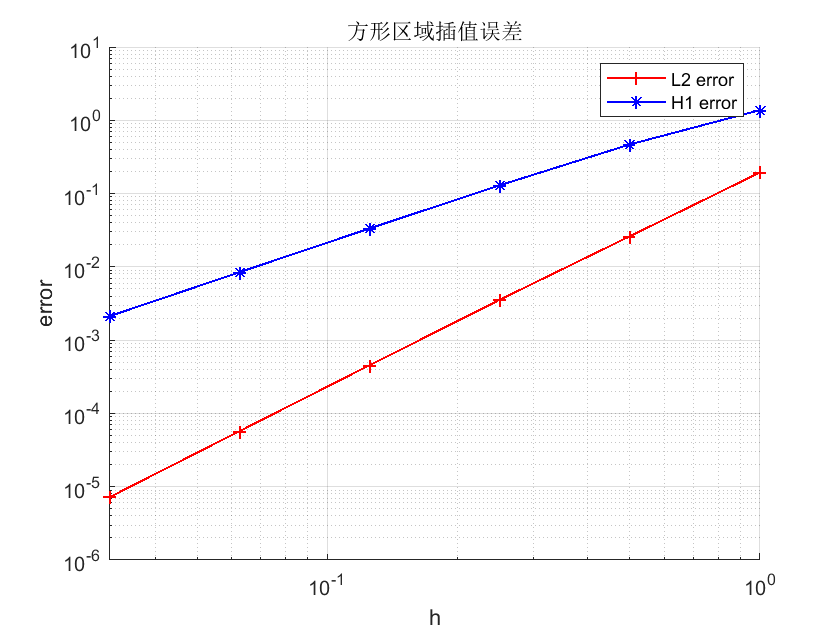
\includegraphics[width=0.9\linewidth]{sqrerror}
		\caption[方形区域误差]{方形区域误差}
		\label{fig:sqrerror}
	\end{figure}
	
	\begin{figure}[h]
		\centering
		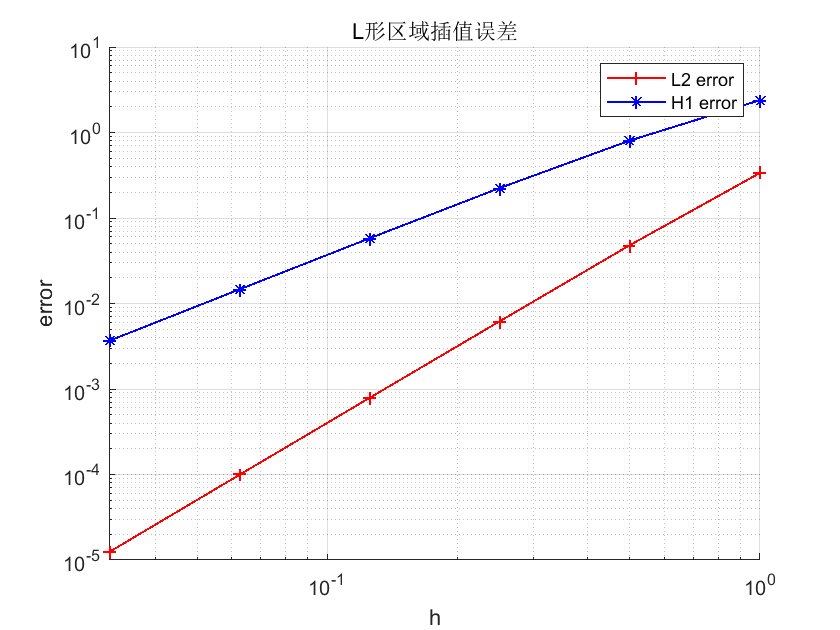
\includegraphics[width=0.9\linewidth]{Lerror}
		\caption[L形区域误差]{L形区域误差}
		\label{fig:Lerror}
	\end{figure}
	
	由结果可知,H1误差收敛阶约为2,L2误差收敛阶约为3.
	
\end{document}

